\subsection{Semantics Equivalence}

Serializability gives us an important consistency property on the \tpl\ operational semantics that we defined. In abstract terms, it allows us to think about program executions in some sequential order, without having to consider all possible interleavings that may arise. At this point, we want to show an even stronger result which is the semantics equivalence between the semantics defined in Section \ref{sec:2plSemantics} and some \textit{atomic} operational semantics, defined in Section \ref{sec:atomicSem}, that reduce transactions in one go, as if the system stops when they begin execution and starts again when they are done. The equivalence not only allows us to forget about the peculiar locking details of \tpl\ and thus only to focus on \textit{atomic} reductions, but also provides us with soundness with respect to the mCAP program logic defined in Section \ref{sec:mcapModel}. This empowers us to build mCAP proofs of programs running under the \tpl\ semantics.

The final outcome of this section will be a proof of the following statement, which says that any program that terminates, i.e. reduces to $\pskip$, under the \tpl\ operational semantics will have the same overall effect on the global storage as the same terminating program running under the \textsc{Atom} semantics and starting with the same state.
\[
	\forall h, h', S, S', \mathds{P} \ldotp
	(h, \emptyset, S, \mathds{P}) \rightarrow^* (h', \emptyset, S', \pskip) \implies 
	(h, \mathds{P}) \tred^* (h', \pskip)
\]

\subsubsection{Atomic semantics}

\label{sec:atomicSem}

The atomic operational semantics shown here are behaviourally equivalent to the ones presented in Section \ref{sec:mcapOpSem}. They are converted to a transition relation for clarity and in order to ease the general proof, since the \tpl\ semantics are also expressed with a comparable structure.

The rules that follow determine a relation between storages under the effect of a program. At the level of programs, they are very similar to the \tpl\ ones, a part from the absence of a lock manager or a transactions stack. These two structures are not needed here, since there is no interleaving which happens as a result of running transactions concurrently. For this reason, there is no need to globally track information about a transaction's internal execution. Note how such behaviour is obtained through the \textsc{AtExec} rule, which reduces a transaction's body at once, by running a multi-step reduction on command $\mathds{C}$ until it hits $\pskip$. Parallelism is again obtained by nondeterministically reducing one of the two programs that are composed together.

\[
(-, -) \rightarrow (-, -) : (\mathsf{Storage} \times \mathsf{Prog})^2
\]
\[\footnotesize\def\arraystretch{3.5}
	\begin{array}{c c}
		\infer[\textsc{AtTrans}]
		{
			(h, \mathds{T}) \tred (h', \pskip)
		}
		{
			(h, \mathds{T}) \tred (h', \ptdef{\pskip})
		}
		&
		\infer[\textsc{AtPSkip}]
		{
			(h, \pskip ; \mathds{P}) \tred (h, \mathds{P})
		}
		{}
		\\
		\infer[\textsc{AtPSeq}]
		{
			(h, \mathds{P}_1 ; \mathds{P}_2) \tred (h', \mathds{P}_1' ; \mathds{P}_2)
		}
		{
			(h, \mathds{P}_1) \tred (h', \mathds{P}_1')
		}
		&
		\infer[\textsc{AtPar}]
		{
			(h, \pskip \| \pskip) \tred (h, \pskip)
		}
		{}
		\\
		\infer[\textsc{AtParL}]
		{
			(h, \mathds{P}_1 \| \mathds{P}_2) \tred (h', \mathds{P}_1' \| \mathds{P}_2)
		}
		{
			(h, \mathds{P}_1) \tred (h', \mathds{P}_1')
		}
		&
		\infer[\textsc{AtParR}]
		{
			(h, \mathds{P}_1 \| \mathds{P}_2) \tred (h', \mathds{P}_1 \| \mathds{P}_2')
		}
		{
			(h, \mathds{P}_2) \tred (h', \mathds{P}_2')
		}
		\\
		\infer[\textsc{AtChoiceL}]
		{
			(h, \mathds{P}_1 + \mathds{P}_2)
			\tred
			(h, \mathds{P}_1)
		}
		{}
		&
		\infer[\textsc{AtChoiceR}]
		{
			(h, \mathds{P}_1 + \mathds{P}_2)
			\tred
			(h, \mathds{P}_2)
		}
		{}
		\\
		\infer[\textsc{AtLoop}]
		{
			(h, \mathds{P}^*)
			\tred
			(h, \pskip + (\mathds{P} ; \mathds{P}^*))
		}
		{}
		&
		\infer[\textsc{AtExec}]
		{
			(h, \ptdef{\mathds{C}})
			\tred
			(h', \ptdef{\pskip})
		}
		{
			(h, \emptyset, \mathds{C})
			\tred^*
			(h', -, \pskip)
		}
	\end{array}
\]

The atomic operational semantics of commands are defined through the rules that follow. They show the reduction of a command when executed on a storage $h$ and variable stack $s$. The rules are equivalent to the \tpl\ ones but, given the atomic setting, there is no need for a state component that determines the phase of a transaction. There are no rules concerned with locking and unlocking either, since under the atomic semantics, transactions run in concrete and real isolation without the need to be managed when accessing storage cells.

\[
(-, -, -) \tred (-, -, -) : (\mathsf{Storage} \times \mathsf{Stack} \times \mathsf{Cmd})^2
\]
\[\footnotesize\def\arraystretch{3.5}
	\begin{array}{@{\hspace*{-20pt}}c @{\hspace{5pt}} c @{}}
		\infer[\textsc{AtSkip}]
		{
			(h, s, \pskip ; \mathds{C})
			\tred
			(h, s, \mathds{C})
		}
		{}
		&
		\infer[\textsc{AtCondT}]
		{
			(h, s, \pif{\mathds{B}}{\mathds{C}_1}{\mathds{C}_2})
			\tred
			(h, s, \mathds{C}_1)
		}
		{
			\llbracket \mathds{B} \rrbracket_s^B = \top
		}
		\\
		\infer[\textsc{AtSeq}]
		{
			(h, s, \mathds{C}_1 ; \mathds{C}_2)
			\tred
			(h', s', \mathds{C}_1' ; \mathds{C}_2)
		}
		{
			(h, s, \mathds{C}_1)
			\tred
			(h', s',\mathds{C}_1')
		}
		&
		\infer[\textsc{AtWrite}]
		{
			(h, s, \pmutate{\mathds{E}_1}{\mathds{E}_2})
			\tred
			(h[k \mapsto v], s, \pskip)
		}
		{
			k = \llbracket \mathds{E}_1 \rrbracket_s\ \
			k \in \pred{dom}{h}\ \
			v = \llbracket \mathds{E}_2 \rrbracket_s
		}
		\\
		\infer[\textsc{AtAssign}]
		{
			(h, s, \passign{\pvar{x}}{\mathds{E}})
			\tred
			(h, s[\pvar{x} \mapsto v], \pskip)
		}
		{
			v = \llbracket \mathds{E} \rrbracket_s
		}
		&
		\infer[\textsc{AtLoopF}]
		{
			(h, s, \ploop{\mathds{B}}{\mathds{C}})
			\tred
			(h, s, \pskip)
		}
		{
			\llbracket \mathds{B} \rrbracket_s^B = \bot
		}
		\\
		\infer[\textsc{AtCondF}]
		{
			(h, s, \pif{\mathds{B}}{\mathds{C}_1}{\mathds{C}_2})
			\tred
			(h, s, \mathds{C}_2)
		}
		{
			\llbracket \mathds{B} \rrbracket_s^B = \bot
		}
		&
		\infer[\textsc{AtRead}]
		{
			(h, s, \pderef{\pvar{x}}{\mathds{E}})
			\tred
			(h, s[\pvar{x} \mapsto v], \pskip)
		}
		{
			k = \llbracket \mathds{E} \rrbracket_s\ \
			k \in \pred{dom}{h}\ \
			v = h(k)
		}
		\\
		\infer[\textsc{AtLoopT}]
		{
			(h, s, \ploop{\mathds{B}}{\mathds{C}})
			\tred
			(h, s, \mathds{C}; \ploop{\mathds{B}}{\mathds{C}})
		}
		{
			\llbracket \mathds{B} \rrbracket_s^B = \top
		}
	\end{array}
\]
\[\footnotesize
\infer[\textsc{AtAlloc}]
{
	(h, s, \palloc{\pvar{x}}{\mathds{E}})
	\tred
	(h[l \mapsto 0] \ldots [l + n - 1 \mapsto 0], s[\pvar{x} \mapsto l], \pskip)
}
{
	n = \llbracket \mathds{E} \rrbracket_s\ \
	l, \ldots, l + n - 1 \not\in \pred{dom}{h}
}
\]

\subsubsection{Trace equivalence}

The final proof of equivalence will need a number of preliminary lemmata in order to succeed. Most of them describe a series of concrete transformations applied to traces that preserve the semantic meaning of the trace in terms of the effects on the global storage. We start by giving some helpful definitions that will be later used as part of the lemmata.

The first one allows to express that a trace $\tau$ is able to generate a particular storage starting from a given initial state with a storage, lock manager, transactions' stack and program components. It serves the purpose of comparing different traces by establishing a type of trace equivalence. In fact, we obtain important information knowing that two distinct traces $\tau$ and $\tau'$ can generate the same heap under specific circumstances.

\begin{defn}
	(Trace generated).
	A trace $\tau$ \emph{generates} a storage $\underline{h}$ starting from the state $h, \Phi, S, \mathds{P}$ if and only if every action in $\tau$ labels one of consecutive reductions that bring $\mathds{P}$ to $\pskip$ under the \tpl\ operational semantics.
	\begin{align*}
		\pred{tgen}{[], h, \underline{h}, \Phi, S, \mathds{P}}
			\iff&
		h = \underline{h} \land \mathds{P} = \pskip \land \Phi = \emptyset
			\\
		\pred{tgen}{(\alpha, n) : \tau, h, \underline{h}, \Phi, S, \mathds{P}}
			\iff&
		\exists h', \Phi', S', \mathds{P}' \ldotp (h, \Phi, S, \mathds{P}) \xrightarrow{\alpha} (h', \Phi', S', \mathds{P}') \\ &\land \pred{tgen}{\tau, h', \underline{h}, \Phi', S', \mathds{P}'}
	\end{align*}
\end{defn}

In order for the \tpl\ operational semantics to model any kind of two phase locking pattern, we utilize nondeterministic locking of storage cells, as described in Section \ref{sec:opSemCmd2pl}. This comes with the downside of allowing a transaction to lock (and later unlock) any cell it wants. Such phenomenon can happen even if later in the execution the same transaction does not use the locks to access the respective storage cells to read from or write to them. Lock operations performed by a transaction as part of a trace, which are never used to later access the corresponding cell are often and informally referred to as \textit{spurious}. The next two definitions formally describe this behaviour.

\begin{defn}
	(Absent access).
	A cell which is neither read or written to by a given transaction as part of a trace is \emph{absent} and the corresponding predicate is defined as follows:
	\[
		\pred{absent}{\iota, k, \tau}
			\iff
		\lnot \exists v, n \ldotp (\actread{\iota}{k}{v}, n) \in \tau \lor (\actwrite{\iota}{k}{v}, n) \in \tau
	\]
\end{defn}

\begin{defn}
	(Clean trace).
	A trace is \emph{clean} if and only if its transactions do not lock or unlock any absent cell.
	\[
		\pred{clean}{\tau} \iff \forall \iota, k, \kappa, n \ldotp
		\left( (\actlock{\iota}{k}{\kappa}, n) \in \tau \lor (\actunlock{\iota}{k}, n) \in \tau \right)
			\implies
		\lnot \pred{absent}{\iota, k, \tau}
	\]
\end{defn}

\begin{center}
	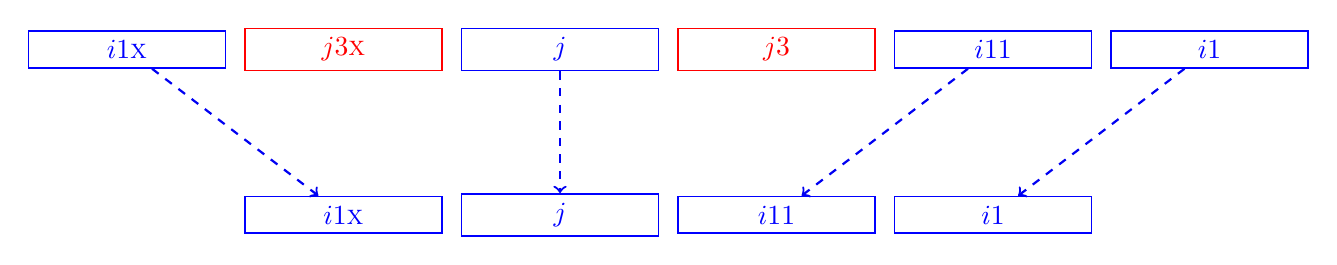
\begin{tikzpicture}[->, semithick]
		\tikzset{
		    tleft/.style= {rectangle, draw=blue, color=blue, minimum width=2.5cm},
		    tright/.style= {rectangle, draw=red, color=red, minimum width=2.5cm},
		    pleft/.style= {above, black!5!blue, thick},
		    pright/.style= {above, black!5!magenta, thick},
		}
		
		\node[tleft] (s1) at (0, 0) {$\actlock{i}{1}{\textsc{x}}$};
		\node[tright] (s2) at (2.75, 0) {$\actlock{j}{3}{\textsc{x}}$};
		\node[tleft] (s3) at (5.5, 0) {$\actid{j}$};
		\node[tright] (s4) at (8.25, 0) {$\actunlock{j}{3}$};
		\node[tleft] (s5) at (11, 0) {$\actwrite{i}{1}{1}$};
		\node[tleft] (s6) at (13.75, 0) {$\actunlock{i}{1}$};
		
		\node[tleft] (s7) at (2.75,-2.1) {$\actlock{i}{1}{\textsc{x}}$};
		\node[tleft] (s8) at (5.5,-2.1) {$\actid{j}$};
		\node[tleft] (s9) at (8.25,-2.1) {$\actwrite{i}{1}{1}$};
		\node[tleft] (s10) at (11,-2.1) {$\actunlock{i}{1}$};
		
		\draw[dashed]
		(s1) edge[pleft] (s7)
		(s3) edge[pleft] (s8)
		(s5) edge[pleft] (s9)
		(s6) edge[pleft] (s10);
	\end{tikzpicture}
	\captionof{figure}{A trace containing spurious locks and its clean equivalent.}
\end{center}

We are able to modify the structure of a trace through the union or the difference with a set of operations, which we formally define as follows.
\begin{defn}
	(Trace difference).
	\[
		\tau' = \tau \setminus S \iff \left( \forall x \ldotp x \not\in S \implies (x \in \tau \iff x \in \tau') \right)
	\]
\end{defn}

\begin{defn}
	(Trace union).
	\begin{gather*}
		\tau' = \tau \cup S \iff \\
		(\forall \alpha, n \ldotp
		(\alpha, n) \in S \implies \left( \lnot \exists \alpha' \ldotp (\alpha', n) \in \tau \right) \\
		\land\ \forall x \ldotp (x \in \tau \lor x \in S) \iff x \in \tau')
	\end{gather*}
\end{defn}

It is now possible to show that any trace $\tau$ that contains a spurious lock (followed by an unlock on the same item) and is able to generate a particular storage $h'$, has a corresponding trace $\tau'$ which contains all of $\tau$'s operations a part from the spurious ones, and $\tau'$ can generate $h'$ starting with the same initial state and program.

\begin{lem}
	(Proof in \ref{lem:lockAbsent}).
	Lock and unlock operations done by a transaction on items which it does not read or write can be removed without affecting the program or the global state.
	\begin{gather*}
		\forall \tau, \tau', h, h', \Phi, S, \mathds{P}, n, n', \iota, k, \kappa, x, y \ldotp
			\\
		\pred{tgen}{\tau, h, h', \Phi, S, \mathds{P}} \land  \pred{absent}{\iota, k, \tau} \land x = (\actlock{\iota}{k}{\kappa}, n) \land y = (\actunlock{\iota}{k}, n') \\ \land x \in \tau \land y \in \tau
		\land \tau' = \tau \setminus \{ x, y \}
			\implies
		\pred{tgen}{\tau', h, h', \Phi, S, \mathds{P}}
	\end{gather*}
\end{lem}

The proof uses another important property of operations inside a trace which is the fact that a lock on an item is not needed for any reductions a part from a read, a write or an unlock action performed by the same transaction on the same item. As we will see later, we leverage this proof in order to \textit{clean} traces from any spurious locks they contain.

\begin{lem}
	(Proof in \ref{lem:alman}).
	\begin{gather*}
		\forall \mathds{P}, \mathds{P}', h, h', \Phi, \Phi', S, S', \alpha, i, k, v, I, \kappa \ldotp \\
		(h, \Phi, S, \mathds{P}) \xrightarrow{\alpha} (h', \Phi', S', \mathds{P}')
			\land
		(\{i\} \uplus I, \kappa) = \Phi(k)
			\land \\
		\alpha \not\in \{ \actread{i}{k}{v}, \actwrite{i}{k}{v}, \actunlock{i}{k} \}
			\implies
		\exists \Phi_m, \Phi_m', I', \kappa', \kappa'' \ldotp \\
		(h, \Phi_m, S, \mathds{P}) \xrightarrow{\alpha} (h', \Phi_m', S, \mathds{P}')
			\land
		\Phi_m = \Phi[k \mapsto (I, \kappa')]
			\land
		\Phi_m' = \Phi'[k \mapsto (I', \kappa'')]
			\land
		\kappa' \leq \textsc{s}
	\end{gather*}
\end{lem}

Once a trace is clean, we can proceed to manipulate it and, under certain cases, swap the order of its operations. Repeating this process, will give us a new trace, syntactically different but semantically equivalent, as observed by its effects on the global heap. This is what we are interested in, given our requirement of simulating a serial trace. Whenever in the following definitions we encounter a term of the shape $\alpha(\iota)$ or $\alpha(\iota, k)$ we actually mean the first projection of their operation-level equivalent, i.e. $op(\iota) \downarrow_1$ and $op(\iota, k) \downarrow_1$ respectively.

\begin{defn}
	(Swapped trace).
	A trace $\tau'$ is the \emph{swapped} version of $\tau$ for some operations $x$ and $y$ if and only if $\tau'$ contains all of $\tau$'s operations in the same exact order a part from the one of $x$ and $y$, which is swapped.
	\begin{gather*}
		\tau' = \pred{swap}{\tau, x, y}
		\iff \\
		\exists \alpha_x, n_x, \alpha_y, n_y \ldotp x = (\alpha_x, n_x) \land y = (\alpha_y, n_y)\ \land \\
		\tau' = \tau \setminus \{(\alpha_x, n_x), (\alpha_y, n_y)\} \cup \{ (\alpha_x, n_y), (\alpha_y, n_x) \}
	\end{gather*}
\end{defn}

We start by showing that the order of two consecutive reads can be swapped as long as the transactions performing them are distinct. Since reads do not alter the storage and they only require at least a shared lock on the target cell, we always succeed in the swap. It is fundamental for the transactions to be different otherwise we would be potentially altering the control flow inside the body of a transaction.
\begin{lem}
	(Proof in \ref{lem:rr}).
	\begin{gather*}
		\forall \tau, \tau', h, h', \Phi, S, \mathds{P}, i, j, k, k', v, v', \alpha, \alpha', n \ldotp \\
		i \neq j \land \alpha = \actread{i}{k}{v} \land \alpha' = \actread{j}{k'}{v'} \land (\alpha, n) \in \tau \land (\alpha', n+1) \in \tau \\ \land\ \pred{tgen}{\tau, h, h', \Phi, S, \mathds{P}} \land \tau' = \pred{swap}{\tau, (\alpha, n), (\alpha', n+1)}
			\\	 
		 \implies \pred{tgen}{\tau', h, h', \Phi, S, \mathds{P}}
	\end{gather*}
\end{lem}

The order of two consecutive read, write, lock or unlock operations can be swapped as long as the transactions performing them are distinct and the keys they refer to are different.
\begin{lem}
	(Proof in \ref{lem:rwlu}).
	\begin{gather*}
		\forall \tau, \tau', h, h', \Phi, S, \mathds{P}, i, j, k, k', x, y, n \ldotp \\
			i \neq j \land x = \alpha(i, k) \land y = \alpha(j, k') \land k \neq k' \land (x, n) \in \tau \land (y, n+1) \in \tau \\ \land\ \pred{tgen}{\tau, h, h', \Phi, S, \mathds{P}} \land \tau' = \pred{swap}{\tau, (x, n), (y, n+1)}
			\\	 
		 \implies \pred{tgen}{\tau', h, h', \Phi, S, \mathds{P}}
	\end{gather*}
\end{lem}

In the case of two consecutive alloc operations inside a trace, we only require for the transactions performing them to be distinct. There is no constraint on the keys generated since we already know they must be two disjoint sets, otherwise the original reduction would have not been allowed.
\begin{lem}
	(Proof in \ref{lem:aa}).
	\begin{gather*}
		\forall \tau, \tau', h, h', \Phi, S, \mathds{P}, i, j, m, m', l, l', \alpha, \alpha', n \ldotp \\
			i \neq j \land \alpha = \actalloc{i}{m}{l} \land \alpha' = \actalloc{j}{m'}{l'} \land (\alpha, n) \in \tau \land (\alpha', n+1) \in \tau \\ \land\ \pred{tgen}{\tau, h, h', \Phi, S, \mathds{P}} \land \tau' = \pred{swap}{\tau, (\alpha, n), (\alpha', n+1)}
			\\	 
		 \implies \pred{tgen}{\tau', h, h', \Phi, S, \mathds{P}}
	\end{gather*}
\end{lem}

We are always able to swap the order of a storage allocation operation followed by a read, write, lock or unlock as long as the transactions performing them are distinct and the keys accessed are not part of the ones created by the allocation. If the latter was not considered as a requirement, then we would allow to access a storage cell which is absent from the heap: an impossible case.
\begin{lem}
	(Proof in \ref{lem:ax}).
	\begin{gather*}
		\forall \tau, \tau', h, h', \Phi, S, \mathds{P}, i, j, k, x, y, n, m, l \ldotp \\
			i \neq j \land x = \alpha(j, k) \land y = \actalloc{i}{m}{l} \land (x, n) \in \tau \land (y, n+1) \in \tau \land (k < l \lor k \geq l + n) \\ \land\ \pred{tgen}{\tau, h, h', \Phi, S, \mathds{P}} \land \tau' = \pred{swap}{\tau, (x, n), (y, n+1)}
			\\	 
		 \implies \pred{tgen}{\tau', h, h', \Phi, S, \mathds{P}}
	\end{gather*}
\end{lem}

The final and simpler case is the one regarding one $\mathsf{id}$ transition. Given that by definition, $\actid{\iota}$ does not affect the global state but it is limited to label control flow reductions within transaction $\mathds{T}_\iota$, the relative order with respect to any other action performed by a different transaction does not matter.
\begin{lem}
	(Proof in \ref{lem:idx}).
	\begin{gather*}
		\forall \tau, \tau', h, h', \Phi, S, \mathds{P}, i, j, x, y, n \ldotp \\
			i \neq j \land x = \actid{i} \land y = \alpha(j) \land (x, n) \in \tau \land (y, n+1) \in \tau \\ \land\ \pred{tgen}{\tau, h, h', \Phi, S, \mathds{P}} \land \tau' = \pred{swap}{\tau, (x, n), (y, n+1)}
			\\	 
		 \implies \pred{tgen}{\tau', h, h', \Phi, S, \mathds{P}}
	\end{gather*}
\end{lem}

The semantically valid swap operations allowed on traces are summarized in the following table, where $\alpha$ and $\alpha'$ label two consecutive operations inside a program trace and the \textit{condition} is the sufficient requirement needed to perform the swap.

\begin{lem}
	(Swap rules).
	\begin{gather*}
		\forall
			\alpha, \alpha',
			i, j, k, \kappa,
			h, h', h_a,
			\Phi, \Phi', \Phi_a,
			S, S', S_a,
			\mathds{P}, \mathds{P}', \mathds{P}_a
		\ldotp \\
		(h, \Phi, S, \mathds{P})
			\xrightarrow{\alpha}
		(h_a, \Phi_a, S_a, \mathds{P}_a)
			\xrightarrow{\alpha'}
		(h', \Phi', S', \mathds{P}')
			\land
			i \neq j \\
			\land
		\lnot \left( \alpha = \actunlock{i}{k}
			\land
		\alpha' = \actlock{j}{k}{\kappa} \right)
			\land
		\alpha = \alpha(i)
			\land
		\alpha' = \alpha(j) \\
			\implies
		\exists h_b, \Phi_b, S_b, \mathds{P}_b \ldotp
		(h, \Phi, S, \mathds{P})
			\xrightarrow{\alpha'}
		(h_b, \Phi_b, S_b, \mathds{P}_b)
			\xrightarrow{\alpha}
		(h', \Phi', S', \mathds{P}')
	\end{gather*}
	\begin{proof}
	Let's pick arbitrary $\alpha, \alpha' \in \mathsf{Act}, i, j \in \mathsf{Tid}, k \in \mathsf{Key}, \kappa \in \mathsf{Lock}, h, h', h_a \in \mathsf{Storage}, \Phi, \Phi', \Phi_a \in \mathsf{LMan}, S, S', S_a \in \mathsf{TState}, \mathds{P}, \mathds{P}', \mathds{P}_a \in \mathsf{Prog}$ and assume that the following holds:
	\begin{gather}
		\label{lem:swapT1}
		(h, \Phi, S, \mathds{P})
			\xrightarrow{\alpha}
		(h_a, \Phi_a, S_a, \mathds{P}_a)
			\xrightarrow{\alpha'}
		(h', \Phi', S', \mathds{P}')
			\land
			i \neq j \\
			\land
		\label{lem:swapT2}
		\lnot \left( \alpha = \actunlock{i}{k}
			\land
		\alpha' = \actlock{j}{k}{\kappa} \right)
			\land
		\alpha = \alpha(i)
			\land
		\alpha' = \alpha(j)
	\end{gather}
	We now proceed in finding $h_b, \Phi_b, S_b, \mathds{P}_b$ by doing a case-by-case analysis on $\alpha$ and $\alpha'$ based on the feasible, i.e. the ones allowed by the \tpl\ operational semantics, reductions they can be part of according to (\ref{lem:swapT1}). From (\ref{lem:swapT2}) we know that neither $\alpha$ nor $\alpha'$ are system transitions $\actprog$. Similarly, we can't have a situation where $\alpha'$ is a lock on a key that was just unlocked by $\alpha$. Also, since from (\ref{lem:swapT1}) we know that $i \neq j$ which implies that, without loss of generality, programs $\mathds{P}, \mathds{P}_a, \mathds{P}'$ have the following shape:
	\[
		\begin{array}{c @{\hspace{15pt}} c @{\hspace{15pt}} c}
			\mathds{P}
				=
			\left( \mathds{T}_i ; \mathds{P}_1 \right)
				\|
			\left( \mathds{T}_j ; \mathds{P}_2 \right)
				\|
			\mathds{P}_3
			&
			\mathds{P}_a
				=
			\left( \mathds{T}_i' ; \mathds{P}_1 \right)
				\|
			\left( \mathds{T}_j ; \mathds{P}_2 \right)
				\|
			\mathds{P}_3
			&
			\mathds{P}'
				=
			\left( \mathds{T}_i' ; \mathds{P}_1 \right)
				\|
			\left( \mathds{T}_j' ; \mathds{P}_2 \right)
				\|
			\mathds{P}_3
		\end{array}
	\]
	Let us also define the new intermediate program, $\dot{\mathds{P}}$, for all the cases we will consider:
	\[
		\dot{\mathds{P}}
			=
		\left( \mathds{T}_i ; \mathds{P}_1 \right)
			\|
		\left( \mathds{T}_j' ; \mathds{P}_2 \right)
			\|
		\mathds{P}_3
	\]
	\begin{enumerate}[label=({\roman*})]
		\item If $\alpha = \actid{i}$ then from the semantic interpretation of $\mathsf{i}$, we obtain that $h_a = h, \Phi_a = \Phi, S_a = S$. It follows that for any action $\alpha'$ performed by $j$ we have the following reduction, from (\ref{lem:swapT1}):
		\[
			(h, \Phi, S, \mathds{P})
				\xrightarrow{\alpha'}
			(h', \Phi', S', \dot{\mathds{P}})
				\xrightarrow{\alpha}
			(h', \Phi', S', \mathds{P}')
		\]
		We can therefore pick $h_b = h', \Phi_b = \Phi', S_b = S'$ and $\mathds{P}_b = \dot{\mathds{P}}$. The same occurs when picking $\alpha' = \actid{j}$ and an arbitrary $\alpha = \alpha(i)$.
		
		\item If $\alpha = \actread{i}{k}{v}$ and $\alpha' = \actread{j}{k'}{v}$ then from the semantic interpretation of $\mathsf{read}$ we know that $h' = h_a = h, \Phi' = \Phi_a = \Phi$. Also, the two $\mathsf{read}$ actions will update transaction-local variables to the values read from the storage so we select $S_b$ to be $S[j \mapsto (s[\pvar{x} \mapsto v], p)]$ where $(s, p) = S(j)$. This implies that we can always reduce in the following way:
		\[
			(h, \Phi, S, \mathds{P})
				\xrightarrow{\alpha'}
			(h, \Phi, S_b, \dot{\mathds{P}})
				\xrightarrow{\alpha}
			(h, \Phi, S', \mathds{P}')
		\]
		We can therefore pick $h_b = h', \Phi_b = \Phi'$ and $\mathds{P}_b = \dot{\mathds{P}}$.
		
		\item If $\alpha = \actread{i}{k}{v}$ and $\alpha' = \actwrite{j}{k'}{v'}$ then from (\ref{lem:swapT1}) it must be the case that $k \neq k'$. This means that given the disjointness of keys, we can always find $h_b = h', \Phi_b = \Phi, S_b = S, \mathds{P}_b = \dot{\mathds{P}}$.
		
		\item If $\alpha = \actwrite{i}{k}{v}$ and $\alpha' = \actwrite{j}{k'}{v'}$ then from (\ref{lem:swapT1}) it must be the case that $k \neq k'$. Now we can always find $h_b = h[k' \mapsto v'], \Phi_b = \Phi, S_b = S, \mathds{P}_b = \dot{\mathds{P}}$.
		
		\item If $\alpha = \actread{i}{k}{v}$ and $\alpha' = \actlock{j}{k'}{\kappa}$ then from (\ref{lem:swapT1}) it must be the case that either $k \neq k'$ or $k = k'$ and $\Phi(k) = (\{i\} \uplus I, \textsc{s})$ and $\kappa = \textsc{s}$. In both cases we can find $h_b = h, \Phi_b = \Phi', S_b = S, \mathds{P}_b = \dot{\mathds{P}}$.
		
		\item If $\alpha = \actwrite{i}{k}{v}$ and $\alpha' = \actlock{j}{k'}{\kappa}$ then from (\ref{lem:swapT1}) it must be the case that $k \neq k'$. Now we can always find $h_b = h, \Phi_b = \Phi', S_b = S, \mathds{P}_b = \dot{\mathds{P}}$.
		
		\item If $\alpha = \actread{i}{k}{v}$ and $\alpha' = \actunlock{j}{k'}$ then from (\ref{lem:swapT1}) it must be the case that either $k \neq k'$ or $k = k'$ and $\Phi(k) = (\{i,j\} \uplus I, \textsc{s})$. In both cases we can find $h_b = h, \Phi_b = \Phi', S_b = S[j \mapsto (s, \pshrink)], \mathds{P}_b = \dot{\mathds{P}}$ for $s = S(j) \downarrow_1$.
		
		\item If $\alpha = \actwrite{i}{k}{v}$ and $\alpha' = \actunlock{j}{k'}$ then from (\ref{lem:swapT1}) it must be the case that $k \neq k'$. Now we can always find $h_b = h, \Phi_b = \Phi', S_b = S', \mathds{P}_b = \dot{\mathds{P}}$.
		
		\item If $\alpha = \actread{i}{k}{v}$ and $\alpha' = \actalloc{j}{n}{l}$ then from (\ref{lem:swapT1}) it must be the case that $k < l \lor l \geq l + n$. Now we can always find $h_b = h', \Phi_b = \Phi', S_b = S[j \mapsto (s[\pvar{x} \mapsto l], p)], \mathds{P}_b = \dot{\mathds{P}}$. Where $\pvar{x}$ is the variable recording the newly allocated address $l$ in transaction $j$ and $(s, p) = S(j)$.
		
		\item If $\alpha = \actwrite{i}{k}{v}$ and $\alpha' = \actalloc{j}{n}{l}$ then from (\ref{lem:swapT1}) it must be the case that $k < l \lor l \geq l + n$. Now we can always find $h_b = h[l \mapsto 0]\ldots[l + n - 1 \mapsto 0], \Phi_b = \Phi', S_b = S[j \mapsto (s[\pvar{x} \mapsto l], p)], \mathds{P}_b = \dot{\mathds{P}}$. Where $\pvar{x}$ is the variable recording the newly allocated address $l$ in transaction $j$ and $(s, p) = S(j)$.
		
		\item If $\alpha = \actlock{i}{k}{\kappa}$ and $\alpha' = \actlock{j}{k'}{\kappa'}$ then from (\ref{lem:swapT1}) it must be the case that either $k \neq k'$ or $k = k'$ and $\kappa = \kappa' = \textsc{s}$. In the first scenario we can find $\Phi_b = \Phi[k' \mapsto (\{j\} \uplus I', \kappa')]$ while in the second one $\Phi_b = \Phi[k \mapsto (\{j\} \uplus I, \textsc{s})]$ with $i \not\in I$. In both cases we pick $h_b = h, S_b = S, \mathds{P}_b = \dot{\mathds{P}}$.
		
		\item If $\alpha = \actunlock{i}{k}$ and $\alpha' = \actunlock{j}{k'}$ then from (\ref{lem:swapT1}) it must be the case that either $k \neq k'$ or $k = k'$ and $\Phi(k) = (\{i, j\} \uplus I, \textsc{s})$. In the first scenario we can find $\Phi_b = \Phi[k' \mapsto (I', \kappa'')]$ for $(\{j\} \uplus I', \kappa') = \Phi(k')$, while in the second one $\Phi_b = \Phi[k \mapsto (\{i\} \uplus I, \textsc{s})]$ with $j \not\in I$. In both cases we pick $h_b = h, S_b = S[j \mapsto (s, \pshrink)], \mathds{P}_b = \dot{\mathds{P}}$. for $s = S(j) \downarrow_1$.
		
		\item If $\alpha = \actlock{i}{k}{\kappa}$ and $\alpha' = \actunlock{j}{k'}$ then from (\ref{lem:swapT1}) it must be the case that either $k \neq k'$ and we find $\Phi_b = \Phi[k' \mapsto (I', \kappa'')]$ for $(\{j\} \uplus I', \kappa') = \Phi(k')$ or $k = k'$ and $\Phi(k) = (\{j\} \uplus I, \textsc{s})$ and $\kappa = \textsc{s}$. In the latter case we can find $\Phi_b = \Phi[k \mapsto (I, \textsc{s})]$. In both cases we pick $h_b = h, S_b = S', \mathds{P}_b = \dot{\mathds{P}}$.
		
		\item If $\alpha = \actunlock{i}{k}$ and $\alpha' = \actlock{j}{k'}{\kappa}$ then from (\ref{lem:swapT2}) it must be the case that $k \neq k'$. Now we can always find $h_b = h, \Phi_b = \Phi[k' \mapsto (\{j\} \uplus I, \kappa)], S_b = S, \mathds{P}_b = \dot{\mathds{P}}$.
		
		\item If $\alpha = \actalloc{i}{n}{l}$ and $\alpha' = \actlock{j}{k}{\kappa}$ then from (\ref{lem:swapT1}) it must be the case that $k < l \lor k \geq l + n$. Now we can always find $h_b = h, \Phi_b = \Phi[k \mapsto (\{j\} \uplus I, \kappa)], S_b = S, \mathds{P}_b = \dot{\mathds{P}}$.
		
		\item If $\alpha = \actalloc{i}{n}{l}$ and $\alpha' = \actunlock{j}{k}$ then from (\ref{lem:swapT1}) it must be the case that $k < l \lor k \geq l + n$. Now we can always find $h_b = h, \Phi_b = \Phi[k \mapsto (I, \kappa')], S_b = S[j \mapsto (s, \pshrink)], \mathds{P}_b = \dot{\mathds{P}}$, for $(\{j\} \uplus I, \kappa) = \Phi(k), \kappa' \leq \textsc{s}$ and $s = S(j) \downarrow_1$.
		
		\item If $\alpha = \actalloc{i}{n}{l}$ and $\alpha' = \actalloc{j}{n'}{l'}$ then from (\ref{lem:swapT1}) it must be the case that $\{l, \ldots, l + n - 1\} \cap \{l', \ldots, l' + n' -1 \} \equiv \emptyset$. Now we can always find $h_b = h[l' \mapsto 0]\ldots[l' + n' - 1 \mapsto 0], \Phi_b = \Phi[l' \mapsto (\{j\}, \textsc{x})]\ldots[l' + n' - 1 \mapsto (\{j\}, \textsc{x})], S_b = S[j \mapsto (s[\pvar{x} \mapsto l'], p)], \mathds{P}_b = \dot{\mathds{P}}$ for $(s, p) = S(j)$.
	\end{enumerate}
	\end{proof}
\end{lem}

\newcolumntype{C}{>{$}c<{$}}
\[\def\arraystretch{1.5}
	\begin{tabular}{|C|C|C|C|}
		\hline
			\alpha
			&
			\alpha'
			&
			\text{Condition} \implies
			&
			\text{Condition} \Longleftarrow
			\\
		\hline
			\actid{i}
			&
			\actid{j}
			&
			\top
			&
			\top
			\\
		\hline
			\actid{i}
			&
			\actalloc{j}{n}{l}
			&
			\top
			&
			\top
			\\
		\hline
			\actid{i}
			&
			\actread{j}{k}{v}
			&
			\top
			&
			\top
			\\
		\hline
			\actid{i}
			&
			\actwrite{j}{k}{v}
			&
			\top
			&
			\top
			\\
		\hline
			\actid{i}
			&
			\actlock{j}{k}{\kappa}
			&
			\top
			&
			\top
			\\
		\hline
			\actid{i}
			&
			\actunlock{j}{k}
			&
			\top
			&
			\top
			\\
		\hline
			\actread{i}{k}{v}
			&
			\actread{j}{k'}{v'}
			&
			\top
			&
			\top
			\\
		\hline
			\actread{i}{k}{v}
			&
			\actwrite{j}{k'}{v'}
			&
			\top
			&
			\top
			\\
		\hline
			\actread{i}{k}{v}
			&
			\actlock{j}{k'}{\kappa}
			&
			\top
			&
			\top
			\\
		\hline
			\actread{i}{k}{v}
			&
			\actunlock{j}{k'}
			&
			\top
			&
			\top
			\\
		\hline
			\actread{i}{k}{v}
			&
			\actalloc{j}{n}{l}
			&
			\top
			&
			k < l \lor k \geq l + n
			\\
		\hline
			\actwrite{i}{k}{v}
			&
			\actwrite{j}{k'}{v'}
			&
			\top
			&
			\top
			\\
		\hline
			\actwrite{i}{k}{v}
			&
			\actlock{j}{k'}{\kappa}
			&
			\top
			&
			\top
			\\
		\hline
			\actwrite{i}{k}{v}
			&
			\actunlock{j}{k'}
			&
			\top
			&
			\top
			\\
		\hline
			\actwrite{i}{k}{v}
			&
			\actalloc{j}{n}{l}
			&
			k < l \lor k \geq l + n
			\\
		\hline
			\actalloc{i}{n}{l}
			&
			\actalloc{j}{n'}{l'}
			&
			\top
			&
			\top
			\\
		\hline
			\actalloc{i}{n}{l}
			&
			\actlock{j}{k}{\kappa}
			&
			k < l \lor k \geq l + n
			&
			\top
			\\
		\hline
			\actalloc{i}{n}{l}
			&
			\actunlock{j}{k}
			&
			k < l \lor k \geq l + n
			&
			\top
			\\
		\hline
			\actlock{i}{k}{\kappa}
			&
			\actlock{j}{k'}{\kappa'}
			&
			\top
			&
			\top
			\\
		\hline
			\actlock{i}{k}{\kappa}
			&
			\actunlock{j}{k'}
			&
			\top
			&
			k \neq k' \lor \kappa = \Phi(k) = \textsc{s}
			\\
		\hline
			\actunlock{i}{k}
			&
			\actunlock{j}{k'}
			&
			\top
			&
			\top
			\\
		\hline
	\end{tabular}
\]

\subsubsection{Strict total order}

\begin{defn}
	(Reflexive image).
	The reflexive image of a set $X$, written $\pred{Id}{X}$, is defined as:
	\[
		\pred{Id}{X} = \{ (x, x)\ |\ x \in X \}
	\]
\end{defn}

\begin{defn}
	(Reflexive closure).
	The reflexive closure of a given relation $R$ on a set $X$, written $R^\mathsf{id}$, is defined as:
	\[
		R^\mathsf{id} = R \cup \pred{Id}{X}
	\]
\end{defn}

\begin{defn}
	(\tpl\ Transactions order)
	\begin{align*}
		\text{let } (N, E) = \pred{SG}{\tau} \text{ in }
		\sqsubset_0 &= E^* \\
		\sqsubset_{n + 1} &=\ \sqsubset_n \cup \left( \sqsubset_n^\mathsf{id} ; \{ (i, j) \} ; \sqsubset_n^\mathsf{id} \right) \\
		&\text{where } i, j \in N \text{ and } i < j \\
		&\text{and } i \not\sqsubset_n j \text{ and } j \not\sqsubset_n i
	\end{align*}
\end{defn}

\begin{thm}
	\label{thm:totOrder}
	(Order of transactions).
	The $\sqsubset$ relation is a strict total order on the set of transactions $N$ in $(N, E) = \pred{SG}{\tau}, \tau = \pred{trace}{h, \emptyset, \emptyset, \mathds{P}}, \mathds{P} \in \mathsf{Prog}, h \in \mathsf{Storage}$.

	\begin{proof}
	In order to show the theorem, we are required to prove that for all $a, b, c \in N$:
	\begin{itemize}
		\item (Irreflexivity). $a \not\sqsubset a$
		\item (Asymmetry). If $a \sqsubset b$ then $b \not\sqsubset a$
		\item (Transitivity). If $a \sqsubset b$ and $b \sqsubset c$ then $a \sqsubset c$
		\item (Totality). $a \sqsubset b$ or $b \sqsubset a$ or $a = b$
	\end{itemize}
	
	Let's pick an arbitrary program $\mathds{P} \in \mathsf{Prog}$, initial storage $h \in \mathsf{Storage}$ and get a trace out of it $\tau = \pred{trace}{h, \emptyset, \emptyset, \mathds{P}}$. We now consider the incrementally built $\sqsubset$ relation on $N$, where $(N, E) = \pred{SG}{\tau}$. \\
	
	(Irreflexivity). The proof follows by induction on the number of $\sqsubset$ relation construction steps, $n$. Let's pick an arbitrary transaction identifier $a \in N$.
	
	{\parindent0pt
	\textit{Base case}: $n = 0$
	
	\textit{To show}: $a \not\sqsubset_0 a$
	
	By definition we know that $\sqsubset_0 = E^*$, i.e. the transitive closure on the edges of the serialization graph $\pred{SG}{\tau}$. We directly obtain that $a \not\sqsubset_0 a$ from Theorem \ref{thm:sgAcyclic}. \\
	
	\textit{Inductive case}: $n > 0$
	
	\textit{Inductive hypothesis}: $a \not\sqsubset_n a$
	
	\textit{To show}: $a \not\sqsubset_{n+1} a$
	
	Let's assume that $a \sqsubset_{n+1} a$ and by definition we know it means that, for some $i, j \in N$ such that $i < j, i \not\sqsubset_n j, j \not\sqsubset_n i$ we have:
	\[
		(a, a) \in \sqsubset_n \cup \left( \sqsubset_n^\mathsf{id} ; \{ (i, j) \} ; \sqsubset_n ^\mathsf{id} \right)
	\]
	and by I.H. we can rewrite it as $(a, a) \in \left( \sqsubset_n^\mathsf{id} ; \{ (i, j) \} ; \sqsubset_n ^\mathsf{id} \right)$ given we assumed that $\sqsubset_n$ is irreflexive. It follows that it must be the case that $(a, i)$ and $(j, a)$ are in $\sqsubset_n^\mathsf{id}$ and moreover they must be in $\sqsubset_n$ given that $i < j$ and therefore $i \neq j$. By transitivity of $\sqsubset_n$, there must be a $(j, i) \in \sqsubset_n$. By contradiction we state that $a \not\sqsubset_{n+1} a$. \\
	}
	
	(Asymmetry). The proof follows by induction on the number of $\sqsubset$ relation construction steps, $n$. Let's pick arbitrary transaction identifiers $a, b \in N$.
	
	{\parindent0pt
	\textit{Base case}: $n = 0$
	
	\textit{To show}: $a \sqsubset_0 b \implies b \not\sqsubset_0 a$
	
	By definition we know that $\sqsubset_0 = E^*$, i.e. the transitive closure on the edges of the serialization graph $\pred{SG}{\tau}$. Let's assume that $a \sqsubset_0 b$ meaning that $a \rightarrow^* b \in E$. We directly obtain that $b \not\sqsubset_0 a$ from Theorem \ref{thm:sgAcyclic}. \\
	
	\textit{Inductive case}: $n > 0$
	
	\textit{Inductive hypothesis}: $a \sqsubset_n b \implies b \not\sqsubset_n a$
	
	\textit{To show}: $a \sqsubset_{n + 1} b \implies b \not\sqsubset_{n + 1} a$
	
	Let's assume that $a \sqsubset_{n + 1} b$ and by definition we know it means that, for some $i, j \in N$ such that $i < j, i \not\sqsubset_n j, j \not\sqsubset_n i$ we have:
	\[
		(a, b) \in \sqsubset_n \cup \left( \sqsubset_n^\mathsf{id} ; \{ (i, j) \} ; \sqsubset_n ^\mathsf{id} \right)
	\]
	\begin{itemize}
		\item If $a \sqsubset_n b$ we know by I.H. that $b \not\sqsubset_n a$. Let's instead assume that $(b, a) \in \left( \sqsubset_n^\mathsf{id} ; \{ (i, j) \} ; \sqsubset_n ^\mathsf{id} \right)$ from which it follows that there is a $(b, i) \in \sqsubset_n^\mathsf{id}$ and $(j, a) \in \sqsubset_n^\mathsf{id}$. By transitivity of $\sqsubset_n$ we obtain that $(j, i) \in \sqsubset_n^\mathsf{id}$ and moreover that $j \sqsubset_n i$ since $i \neq j$ as $i < j$. By contradiction we obtain that $(b, a) \not\in \left( \sqsubset_n^\mathsf{id} ; \{ (i, j) \} ; \sqsubset_n ^\mathsf{id} \right)$. We conclude that $b \not\sqsubset_{n + 1} a$.
		\item If $(a, b) \in \left( \sqsubset_n^\mathsf{id} ; \{ (i, j) \} ; \sqsubset_n ^\mathsf{id} \right)$ which means there is a $(a, i) \in \sqsubset_n^\mathsf{id}$ and $(j, b) \in \sqsubset_n^\mathsf{id}$. Let's now assume that $(b, a) \in \left( \sqsubset_n^\mathsf{id} ; \{ (i, j) \} ; \sqsubset_n ^\mathsf{id} \right)$ meaning that there is a $(b, i) \in \sqsubset_n^\mathsf{id}$ and $(j, a) \in \sqsubset_n^\mathsf{id}$. By transitivity of $\sqsubset_n$ we obtain that $(j, i) \in \sqsubset_n^\mathsf{id}$ and moreover that $j \sqsubset_n i$ since $i \neq j$ as $i < j$. By contradiction we obtain that $(b, a) \not\in \left( \sqsubset_n^\mathsf{id} ; \{ (i, j) \} ; \sqsubset_n ^\mathsf{id} \right)$. We now assume that $b \sqsubset_n a$ which implies that $(b, a) \in \sqsubset_n^\mathsf{id}$. By transitivity of $\sqsubset_n$ we obtain that $(j, i) \in \sqsubset_n^\mathsf{id}$ and moreover that $j \sqsubset_n i$ since $i \neq j$ as $i < j$. By contradiction we obtain that $(b, a) \not\in \sqsubset_n$. We conclude that $b \not\sqsubset_{n + 1} a$.
	\end{itemize}
	}
	
	(Transitivity). We are required to show that $\forall m \geq 1 \ldotp \sqsubset^m\ \subseteq\ \sqsubset$ The proof follows by induction on the number of self-composition steps, $m$.
	
	{\parindent0pt
	\textit{Base case}: $m = 1$
	
	\textit{To show}: $\sqsubset^1\ \subseteq\ \sqsubset$ \\
	
	The result follows directly by definition $\sqsubset^1\ =\ \sqsubset\ \subseteq\ \sqsubset$. \\
	
	\textit{Inductive case}: $m > 1$
	
	\textit{Inductive hypothesis}: $\sqsubset^m\ \subseteq\ \sqsubset$
	
	\textit{To show}: $\sqsubset^{m + 1}\ \subseteq\ \sqsubset$
	\begin{align*}
		\sqsubset^{m + 1}
		&=\ \sqsubset^m ; \sqsubset \text{ by associativity} \\
		&\subseteq\ \sqsubset ; \sqsubset \text{ by I.H.} \\
		&=\ \sqsubset^2 \text{by definition} \\
		&\subseteq\ \sqsubset \text{ by Lemma \ref{lem:total2}}
	\end{align*}
	}
	
	(Totality). Let's pick arbitrary transaction identifiers $a, b \in N$ (\textsc{i}) for a finite $N$ and build the $\sqsubset$ relation on it until convergence, i.e. in a finite number of steps. If $(a, b) \in E^*$ or $(b, a) \in E*$ then we know that either $a \sqsubset b$ or $b \sqsubset a$ holds. On the other hand if there is no edge connecting $a$ to $b$ or $b$ to $a$ in $E^*$ (\textsc{ii}) then:
	\begin{itemize}
		\item If $a = b$ then by irreflexivity of $\sqsubset$ we are done, as totality is met.
		\item Without loss of generality, we say that $a < b$ (\textsc{iii}). Given that the construction of $\sqsubset$ terminated in some $m > 0$ steps (being $N$ a finite set), by (\textsc{i}), (\textsc{ii}) and (\textsc{iii}) we know that there must exist a construction step $n$ such that $0 < n < m$ where the tuple $(a, b)$ was inserted in the relation given that $\sqsubset_{n-1} \cup \left( \sqsubset_{n-1}^\mathsf{id} ; \{(a,b)\} ; \sqsubset_{n-1}^\mathsf{id} \right) \implies a \sqsubset_n b \implies a \sqsubset b$. 
	\end{itemize}
	\end{proof}
\end{thm}
	
\begin{lem}
	\label{lem:total2}
	Given a serialization graph $(N, E) = \pred{SG}{\tau}$ for $\tau = \pred{trace}{h, \emptyset, \emptyset, \mathds{P}}, \mathds{P} \in \mathsf{Prog}, h \in \mathsf{Storage}$, and the $\sqsubset$ relation on the set $N$ we say that $\sqsubset^2\ \subseteq\ \sqsubset$.
	
	{\parindent0pt
	\begin{proof}
	We proceed by induction on the number of $\sqsubset$ construction steps, $n$. \\
	
	\textit{Base case}: $n = 0$
	
	\textit{To show}: $\sqsubset_0^2\ \subseteq\ \sqsubset_0$
	
	By definition we know that $\sqsubset_0 = E^*$, i.e. the transitive closure on the edges of the serialization graph $\pred{SG}{\tau}$. It follows that by definition of transitive closure, $\sqsubset_0^2\ = E^* ; E^* = E^*$ meaning that $\sqsubset_0^2\ \subseteq\ \sqsubset_0$. \\
	
	\textit{Inductive case}: $n > 0$
	
	\textit{Inductive hypothesis}: $\sqsubset_n^2\ \subseteq\ \sqsubset_n$
	
	\textit{To show}: $\sqsubset_{n + 1}^2\ \subseteq\ \sqsubset_{n + 1}$
	
	We can rewrite the formula to be proven as the following, for some $i, j \in N$ such that $i < j, i \not\sqsubset_n j, j \not\sqsubset_n i$:
	\begin{align}
		\left( \sqsubset_n \cup \underbrace{\left( \sqsubset_n^\mathsf{id} ; \{ (i, j) \} ; \sqsubset_n^\mathsf{id} \right)}_{R} \right) ; \left( \sqsubset_n \cup \left( \sqsubset_n^\mathsf{id} ; \{ (i, j) \} ; \sqsubset_n^\mathsf{id} \right) \right) &\subseteq \sqsubset_{n + 1} \\
		\label{thm:total1} \sqsubset_n ; \sqsubset_n \cup \sqsubset_n ; R \cup R ; \sqsubset_n \cup R ; R &\subseteq\ \sqsubset_{n + 1} \text{ by distributivity}
	\end{align}
	It now suffices to show that each unioned set in the L.H.S. of (\ref{thm:total1}) is a subset of $\sqsubset_{n + 1}$ itself.
	\begin{itemize}
		\item \textit{To show}: $\sqsubset_n ; \sqsubset_n\ \subseteq\ \sqsubset_{n + 1}$
			\begin{align}
				\sqsubset_n ; \sqsubset_n\ &=\ \sqsubset_n^2 \\
				\text{by I.H.}&\subseteq\ \sqsubset_n\ \subseteq\ \sqsubset_{n + 1}
			\end{align}
		\item \textit{To show}: $\sqsubset_n ; \left( \sqsubset_n^\mathsf{id} ; \{ (i, j) \} ; \sqsubset_n^\mathsf{id} \right) \subseteq\ \sqsubset_{n + 1}$
			\begin{align}
				S  &=\ \sqsubset_n ; \sqsubset_n^\mathsf{id} \\
					&=\ \sqsubset_n ; \left( \sqsubset_n \cup\ \pred{Id}{N} \right) \text{by definition} \\
					&=\ \sqsubset_n ; \sqsubset_n \cup \sqsubset_n ; \pred{Id}{N} \\
					&=\ \sqsubset_n^2 \cup \sqsubset_n \\
					&\subseteq\ \sqsubset_n \text{by I.H.} \\
					\label{thm:total2} &\subseteq\ \sqsubset_n^\mathsf{id} \text{by definition} \\
				\sqsubset_n ; \left( \sqsubset_n^\mathsf{id} ; \{ (i, j) \} ; \sqsubset_n^\mathsf{id} \right) &= \left( \sqsubset_n ; \sqsubset_n^\mathsf{id} ; \{ (i, j) \} \right) ; \sqsubset_n^\mathsf{id} \text{ by associativity} \\
				&= \left( S ; \{ (i, j) \} \right) ; \sqsubset_n^\mathsf{id} \text{ by associativity} \\
				&\subseteq\ \sqsubset_n^\mathsf{id} ; \{ (i, j) \} ; \sqsubset_n^\mathsf{id} \text{by (\ref{thm:total2})} \\
				&\subseteq\ \sqsubset_{n + 1}
			\end{align}
		\item \textit{To show}: $\left( \sqsubset_n^\mathsf{id} ; \{ (i, j) \} ; \sqsubset_n^\mathsf{id} \right) ; \sqsubset_n \subseteq\ \sqsubset_{n + 1}$
			\begin{align}
				S' &=\ \sqsubset_n^\mathsf{id} ; \sqsubset_n \\
					&= \left( \sqsubset_n \cup\ \pred{Id}{N} \right) ; \sqsubset_n \text{by definition} \\
					&=\ \sqsubset_n ; \sqsubset_n \cup\ \pred{Id}{N} ; \sqsubset_n \\
					&=\ \sqsubset_n^2 \cup \sqsubset_n \\
					&\subseteq\ \sqsubset_n \text{by I.H.} \\
					\label{thm:total3} &\subseteq\ \sqsubset_n^\mathsf{id} \text{by definition} \\
				\left( \sqsubset_n^\mathsf{id} ; \{ (i, j) \} ; \sqsubset_n^\mathsf{id} \right) ; \sqsubset_n &=\ \sqsubset_n^\mathsf{id} ; \left( \{ (i, j) \} ; \sqsubset_n^\mathsf{id} ; \sqsubset_n \right) \text{ by associativity} \\
				&=\ \sqsubset_n^\mathsf{id} ; \left( \{ (i, j) \} ; S' \right) \text{ by associativity} \\
				&\subseteq\ \sqsubset_n^\mathsf{id} ; \{ (i, j) \} ; \sqsubset_n^\mathsf{id} \text{by (\ref{thm:total3})} \\
				&\subseteq\ \sqsubset_{n + 1}
			\end{align}
		\item \textit{To show}: $\left( \sqsubset_n^\mathsf{id} ; \{ (i, j) \} ; \sqsubset_n^\mathsf{id} \right) ; \left( \sqsubset_n^\mathsf{id} ; \{ (i, j) \} ; \sqsubset_n^\mathsf{id} \right) \subseteq\ \sqsubset_{n + 1}$
		
			Let's assume that $\left( \sqsubset_n^\mathsf{id} ; \{ (i, j) \} ; \sqsubset_n^\mathsf{id} \right) ; \left( \sqsubset_n^\mathsf{id} ; \{ (i, j) \} ; \sqsubset_n^\mathsf{id} \right) \neq \emptyset$ meaning that the set at least contains a tuple $(a, b)$, for $a, b \in N$. 
			\begin{align}
				(a, b) \in \left( \sqsubset_n^\mathsf{id} ; \{ (i, j) \} ; \sqsubset_n^\mathsf{id} \right) ; \left( \sqsubset_n^\mathsf{id} ; \{ (i, j) \} ; \sqsubset_n^\mathsf{id} \right)
					&\iff \\
				\exists c \ldotp (a, c) \in \left( \sqsubset_n^\mathsf{id} ; \{ (i, j) \} ; \sqsubset_n^\mathsf{id} \right) \land (c, b) \in \left( \sqsubset_n^\mathsf{id} ; \{ (i, j) \} ; \sqsubset_n^\mathsf{id} \right)
					&\iff \\
				\exists c \ldotp (a, i) \in\ \sqsubset_n^\mathsf{id} \land (i, j) \in  \{(i, j)\} \land (j, c) \in\ \sqsubset_n^\mathsf{id} \\ \land (c, i) \in\ \sqsubset_n^\mathsf{id} \land (i, j) \in  \{(i, j)\} \land (j, b) \in\ \sqsubset_n^\mathsf{id}
					&\implies \\
				\label{thm:total4} \exists c \ldotp (j, c) \in\ \sqsubset_n^\mathsf{id} \land (c, i) \in\ \sqsubset_n^\mathsf{id}
			\end{align}
			We know that $i \neq j$ since $i < j$ so the proof proceeds with a case-by-case analysis on $c$.
			\begin{itemize}
				\item If $c = i$ then we know that $c \neq j$ and by (\ref{thm:total4}) we have that $(j, i) \in\ \sqsubset_n^\mathsf{id} \land (i, i) \in\ \sqsubset_n^\mathsf{id}$ from which it follows that $(j, i) \in\ \sqsubset_n$, a contradiction.
				\item If $c = j$ then we know that $c \neq i$ and by (\ref{thm:total4}) we have that $(j, j) \in\ \sqsubset_n^\mathsf{id} \land (j, i) \in\ \sqsubset_n^\mathsf{id}$ from which it follows that $(j, i) \in\ \sqsubset_n$, a contradiction.
				\item If $c \neq i$ and $c \neq j$ then (\ref{thm:total4}) it follows that $(j, c) \in\ \sqsubset_n \land (c, i) \in\ \sqsubset_n$. By I.H. we know that $\sqsubset_n^2\ \subseteq\ \sqsubset_n$. By definition we know that if $(j, c) \in\ \sqsubset_n$ and $(c, i) \in\ \sqsubset_n$ then $(j, i) \in\ \sqsubset_n^2$. By I.H. this means that $(j, i) \in\ \sqsubset_n$ which is again a contradiction.
			\end{itemize}
			By contradiction we conclude that $\left( \sqsubset_n^\mathsf{id} ; \{ (i, j) \} ; \sqsubset_n^\mathsf{id} \right) ; \left( \sqsubset_n^\mathsf{id} ; \{ (i, j) \} ; \sqsubset_n^\mathsf{id} \right) = \emptyset$ meaning that $\left( \sqsubset_n^\mathsf{id} ; \{ (i, j) \} ; \sqsubset_n^\mathsf{id} \right) ; \left( \sqsubset_n^\mathsf{id} ; \{ (i, j) \} ; \sqsubset_n^\mathsf{id} \right) \subseteq\ \sqsubset_{n + 1}$.
			
			Direct proof.
			\begin{align*}
				\{ (i, j) \} ; \sqsubset_n^\mathsf{id} ; \{ (i, j) \}
					&=
				\{ (i, j) \} ; \left( \sqsubset_n \cup \pred{Id}{N} \right) ; \{ (i, j) \} \\
					&=
				\{ (i, j) \} ; \left( \sqsubset_n ; \{ (i, j) \} \cup \{ (i, j) \} \right) \\
					&=
				\left( \{ (i, j) \} ; \sqsubset_n ; \{ (i, j) \} \right) \cup \left(\{ (i, j) \} ; \{ (i, j) \} \right) \\
				 	&=
				 \left( \{ (i, j) \} ; \sqsubset_n ; \{ (i, j) \} \right) = \emptyset \\
				\left( \sqsubset_n^\mathsf{id} ; \{ (i, j) \} ; \sqsubset_n^\mathsf{id} \right) ; \left( \sqsubset_n^\mathsf{id} ; \{ (i, j) \} ; \sqsubset_n^\mathsf{id} \right)
					&=
				\left( \sqsubset_n^\mathsf{id} ; \{ (i, j) \} \right) ; \left( \sqsubset_n^\mathsf{id} ; \left( \sqsubset_n^\mathsf{id} ; \{ (i, j) \} ; \sqsubset_n^\mathsf{id} \right) \right) \\
					&=
				\left( \sqsubset_n^\mathsf{id} ; \{ (i, j) \} \right) ; \left( \left( \sqsubset_n^\mathsf{id} ;  \sqsubset_n^\mathsf{id} \right) ; \left( \{ (i, j) \} ; \sqsubset_n^\mathsf{id} \right) \right) \\
					&=
				\left( \sqsubset_n^\mathsf{id} ; \{ (i, j) \} \right) ; \left( \sqsubset_n^\mathsf{id} ; \left( \{ (i, j) \} ; \sqsubset_n^\mathsf{id} \right) \right) \\
					&=\
				\sqsubset_n^\mathsf{id} ; \left( \{ (i, j) \} ; \sqsubset_n^\mathsf{id} ; \{ (i, j) \} \right) ; \sqsubset_n^\mathsf{id} \\
					&=\
				\sqsubset_n^\mathsf{id} ; \emptyset ; \sqsubset_n^\mathsf{id} = \emptyset
			\end{align*}
	\end{itemize}
	\end{proof}
	}
\end{lem}

\subsubsection{Proof}

We are ready to tackle the general proof which allows us to show that any full program reduction that happens under \tpl\ semantics can be replicated by the \textsc{Atom} one. This relation will be verified with regards to the final storage achieved by the reductions under the two different semantics. The first level of proof is an induction on the syntactic structure of programs.

The single transaction case $\ptdef{\mathds{C}}$ follows from the single step equivalence of the two operational semantics when reducing sequential commands (i.e. the transaction's body $\mathds{C}$). In the case of a loop $\mathds{P}^*$ and of nondeterministic choice $\mathds{P}_1 + \mathds{P}_2$ we get the needed result from the inductive hypothesys on $\mathds{P}$ and $\mathds{P}_1, \mathds{P}_2$ respectively. The sequential composition of programs is dealt with using a series of auxiliary lemmata together with the inductive hypothesis on $\mathds{P}_1, \mathds{P}_2$. Parallel composition is, as expected, the most challenging case, and its proof requires a particular multi-step strategy summarized at an intuitive level below.
\begin{enumerate}
	\item Retrieve a full trace $\tau$ from the terminating reduction of $\mathds{P}_1 \| \mathds{P}_2$.
	
	\item Clean $\tau$ from any spurious locks that appear inside of it in order to obtain $\tau'$.
	
	\item Convert any redundant exclusive lock in $\tau'$ into a shared one and compute $\tau_{c}$.
	
	\item Build a serialization graph out of $\tau_{c}$.
	
	\item Extend the serialization graph to the strict total order $\sqsubset$ and find its minimal element $\iota$.
	
	\item Swap all of $\iota$'s operations to the left of the trace until no swap is possible anymore. The final trace will be $\tau_{seq}$.
	
	\item Show that no operation done by another transaction can appear in $\tau_{seq}$ before one done by $\iota$.
\end{enumerate}

\begin{thm}

\label{thm:atom}

\[
	\forall h, h', S, S' \ldotp
	(h, \emptyset, S, \mathds{P}) \rightarrow^* (h', \emptyset, S', \pskip) \implies 
	(h, \mathds{P}) \tred^* (h', \pskip)
\]

{\parindent0pt
\begin{proof}
The proof is done by induction on the structure of programs $\mathsf{Prog}$. \\

\textit{Base case 1}: $\pskip \in \mathsf{Prog}$

\textit{To show}:
\[
	\forall h, h', S, S' \ldotp
	(h, \emptyset, S, \pskip) \rightarrow^* (h', \emptyset, S', \pskip) \implies 
	(h, \pskip) \tred^* (h', \pskip)
\]

For arbitrary $h, h', S, S'$ we assume that $(h, \emptyset, S, \pskip) \rightarrow^* (h', \emptyset, S', \pskip)$ holds, and given that $\pskip$ has no possible one-step reductions, it must be the case that it is a zero-step reduction. Therefore we have $h = h'$ and $S = S'$. Starting from $(h, \pskip)$ through the $\tred$ relation, we can always reach $(h, \pskip)$ via a zero-step reduction $(h, \pskip) \tred^0 (h, \pskip)$. We can conclude that $(h, \emptyset, S, \pskip) \rightarrow^* (h', \emptyset, S', \pskip) \implies (h, \pskip) \tred^* (h', \pskip)$ where $h = h'$. \\

\textit{Base case 2}: $\mathds{T} \in \mathsf{Prog}$

\textit{To show}:
\[
	\forall h, h', S, S' \ldotp
	(h, \emptyset, S, \mathds{T}) \rightarrow^* (h', \emptyset, S', \pskip) \implies 
	(h, \mathds{T}) \tred^* (h', \pskip)
\]

We will proceed with the proof by induction on the structure of transactions $\mathsf{Trans}$. Given that the \textsc{Atom} semantics only support user transactions, all that is required to show is:
\begin{gather*}
	\forall h, h', S, S' \ldotp \\
	(h, \emptyset, S, \ptdef{\mathds{C}}) \rightarrow^* (h', \emptyset, S', \pskip) \implies 
	(h, \ptdef{\mathds{C}}) \tred^* (h', \pskip)
\end{gather*}

For arbitrary $h, h', S, S'$ we assume that $(h, \emptyset, S, \ptdef{\mathds{C}}) \rightarrow^* (h', \emptyset, S', \pskip)$ holds. Given the overall reduction from $\ptdef{\mathds{C}}$ to $\pskip$ it must be the case that the following holds.
\begin{gather*}
	(h, \emptyset, S, \ptdef{\mathds{C}})
	\xrightarrow{\actid{\iota}} (h, \emptyset, S[\iota \mapsto (\emptyset, \pgrow)], \ptdef{\mathds{C}}_\iota) \\
	\rightarrow^* (h', \emptyset, S', \ptdef{\pskip}_\iota)
	\xrightarrow{\actprog} (h', \emptyset, S', \pskip)
\end{gather*}
Which implies that $\mathds{C}$ reduces to $\pskip$ through the repeated use of the \textsc{Exec} rule. From the transitive closure of the $\rightarrow$ relation and Lemma \ref{lem:catom} we obtain the result that $(h, \ptdef{\mathds{C}}) \tred^* (h', \pskip)$. \\

\textit{Inductive case 1}: $\mathds{P}_1 + \mathds{P}_2 \in \mathsf{Prog}$

\textit{To show}:
\[
	\forall h, h', S, S' \ldotp
	(h, \emptyset, S, \mathds{P}_1 + \mathds{P}_2) \rightarrow^* (h', \emptyset, S', \pskip) \implies 
	(h, \mathds{P}_1 + \mathds{P}_2 ) \tred^* (h', \pskip)
\]

\textit{Inductive hypothesis}:
\begin{gather*}
	\forall h, h', S, S' \ldotp
	(h, \emptyset, S, \mathds{P}_1) \rightarrow^* (h', \emptyset, S', \pskip) \implies 
	(h, \mathds{P}_1) \tred^* (h', \pskip)
	\\ \land \\
	\forall h, h', S, S' \ldotp
	(h, \emptyset, S, \mathds{P}_2) \rightarrow^* (h', \emptyset, S', \pskip) \implies 
	(h, \mathds{P}_2) \tred^* (h', \pskip)
\end{gather*}

For arbitrary $h, h', S, S'$ we assume that $(h, \emptyset, S, \mathds{P}_1 + \mathds{P}_2) \rightarrow^* (h', \emptyset, S', \pskip)$ holds. Now we are presented with two cases:
\begin{enumerate}
	\item We can reduce $(h, \emptyset, S, \mathds{P}_1 + \mathds{P}_2) \xrightarrow{\actprog} (h, \emptyset, S, \mathds{P}_1)$ with one step through the \textsc{ChoiceL} rule, which we can always apply since it has an empty premiss. We can also always reduce $(h, \mathds{P}_1 + \mathds{P}_2) \tred (h, \mathds{P}_1)$ through the rule \textsc{AtChoiceL} given it has an empty premiss. By inductive hypothesis on $\mathds{P}_1$ we obtain that $(h, \emptyset, S, \mathds{P}_1) \rightarrow^* (h', \emptyset, S', \pskip) \implies (h, \mathds{P}_1) \tred^* (h', \pskip)$. Therefore we can conclude that $(h, \emptyset, S, \mathds{P}_1 + \mathds{P}_2) \rightarrow^* (h', \emptyset, S', \pskip) \implies  (h, \mathds{P}_1 + \mathds{P}_2) \tred^* (h', \pskip)$.
	
	\item We can reduce $(h, \emptyset, S, \mathds{P}_1 + \mathds{P}_2) \xrightarrow{\actprog} (h, \emptyset, S, \mathds{P}_2)$ with one step through the \textsc{ChoiceR} rule, which we can always apply since it has an empty premiss. We can also always reduce $(h, \mathds{P}_1 + \mathds{P}_2) \tred (h, \mathds{P}_2)$ through the rule \textsc{AtChoiceR} given it has an empty premiss. By inductive hypothesis on $\mathds{P}_2$ we obtain that $(h, \emptyset, S, \mathds{P}_2) \rightarrow^* (h', \emptyset, S', \pskip) \implies (h, \mathds{P}_2) \tred^* (h', \pskip)$. Therefore we can conclude that $(h, \emptyset, S, \mathds{P}_1 + \mathds{P}_2) \rightarrow^* (h', \emptyset, S', \pskip) \implies  (h, \mathds{P}_1 + \mathds{P}_2) \tred^* (h', \pskip)$. \\
\end{enumerate}

\textit{Inductive case 2}: $\mathds{P}_1 ; \mathds{P}_2 \in \mathsf{Prog}$

\textit{To show}:
\[
	\forall h, h', S, S' \ldotp
	(h, \emptyset, S, \mathds{P}_1 ; \mathds{P}_2) \rightarrow^* (h', \emptyset, S', \pskip) \implies 
	(h, \mathds{P}_1 ; \mathds{P}_2 ) \tred^* (h', \pskip)
\]

\textit{Inductive hypothesis}:
\begin{gather*}
	\forall h, h', S, S' \ldotp
	(h, \emptyset, S, \mathds{P}_1) \rightarrow^* (h', \emptyset, S', \pskip) \implies 
	(h, \mathds{P}_1) \tred^* (h', \pskip)
	\\ \land \\
	\forall h, h', S, S' \ldotp
	(h, \emptyset, S, \mathds{P}_2) \rightarrow^* (h', \emptyset, S', \pskip) \implies 
	(h, \mathds{P}_2) \tred^* (h', \pskip)
\end{gather*}

For arbitrary $h, h', S, S'$ we assume that $(h, \emptyset, S, \mathds{P}_1 ; \mathds{P}_2) \rightarrow^* (h', \emptyset, S', \pskip)$ holds. Given the overall reduction from $\mathds{P}_1 ; \mathds{P}_2$ to $\pskip$ we must have a chain of reductions of the following shape, for some $h'', S''$: \iffalse where $\Phi'' = \emptyset$ by Lemma \ref{ref:phiemp}. \fi
\[
	\underbrace{(h, \emptyset, S, \mathds{P}_1 ; \mathds{P}_2) \rightarrow^* (h'', \emptyset, S'', \pskip; \mathds{P}_2)}_{(\textsc{i})}
	\xrightarrow{\actprog} (h'', \emptyset, S'', \mathds{P}_2) \rightarrow^* (h', \emptyset, S', \pskip)
\]
\begin{enumerate}
	\item \label{seq:1} By (\textsc{i}) and Lemma \ref{ref:2seq} we get that $(h, \emptyset, S, \mathds{P}_1) \rightarrow^* (h'', \emptyset, S'', \pskip)$ holds.
	
	\item \label{seq:2} By \ref{seq:1}. and the inductive hypothesis on $\mathds{P}_1$ we obtain that $(h, \mathds{P}_1) \tred^* (h'', \pskip)$.
	
	\item By \ref{seq:2}. and Lemma \ref{ref:aseq} we get that $(h, \mathds{P}_1 ; \mathds{P}_2) \tred^* (h'', \pskip ; \mathds{P}_2)$.
\end{enumerate}

At this point we can apply the \textsc{PSeqSkip} rule to reduce $(h'', \emptyset, S'', \pskip ; \mathds{P}_2) \xrightarrow{\actprog} (h'', \emptyset, S'', \mathds{P}_2)$ and rule \textsc{AtPSeqSkip} to reduce $(h'', \pskip ; \mathds{P}_2) \tred^* (h'', \mathds{P}_2)$. By inductive hypothesis on $\mathds{P}_2$ we can conclude that $(h, \emptyset, S, \mathds{P}_1 ; \mathds{P}_2) \rightarrow^* (h', \emptyset, S', \pskip) \implies (h, \mathds{P}_1 ; \mathds{P}_2) \tred^* (h', \pskip)$. \\

\textit{Inductive case 3}: $\mathds{P}^* \in \mathsf{Prog}$

\textit{To show}:
\[
	\forall h, h', S, S' \ldotp
	(h, \emptyset, S, \mathds{P}^*) \rightarrow^* (h', \emptyset, S', \pskip) \implies 
	(h, \mathds{P}^* ) \tred^* (h', \pskip)
\]

\textit{Inductive hypothesis}:
\[
	\forall h, h', S, S' \ldotp
	(h, \emptyset, S, \mathds{P}) \rightarrow^* (h', \emptyset, S', \pskip) \implies 
	(h, \mathds{P}) \tred^* (h', \pskip)
\]

For arbitrary $h, h', S, S'$ we assume that $(h, \emptyset, S, \mathds{P}^*) \rightarrow^* (h', \emptyset, S', \pskip)$ holds (\textsc{i}). Given the overall reduction from $\mathds{P}^*$ to $\pskip$ we must have a chain of reductions of the following shape, for some $h'', \Phi'', S''$:
\[
(h, \emptyset, S, \mathds{P}^*) \rightarrow^* (h'', \Phi'', S'', \pskip + (\mathds{P} ; \mathds{P}^*)) \rightarrow^*  (h', \emptyset, S', \pskip + (\mathds{P} ; \mathds{P}^*)) \xrightarrow{\actprog} (h', \emptyset, S', \pskip)
\]
Through the \textsc{Loop} rule (\textsc{ii}), we can always reduce $(h, \emptyset, S, \mathds{P}^*) \xrightarrow{\actprog} (h, \emptyset, S, \pskip + (\mathds{P} ; \mathds{P}^*))$ given that it has an empty premiss. Similarly, we can always reduce any $(h'', \mathds{P}^*) \tred (h'', \pskip + (\mathds{P} ; \mathds{P}^*))$ via the \textsc{AtLoop} rule as it also has an empty premiss. We now consider two possible cases:
\begin{enumerate}
	\item \label{loop:1} We reduce $(h, \emptyset, S, \pskip + (\mathds{P} ; \mathds{P}^*)) \xrightarrow{\actprog} (h, \emptyset, S, \pskip)$ through the \textsc{ChoiceL} rule which we can always do, together with \textsc{AtChoiceL} that reduces $(h, \pskip + (\mathds{P} ; \mathds{P}^*)) \tred (h, \pskip)$. In this scenario we directly obtain the result.
	
	\item We reduce $(h, \emptyset, S, \pskip + (\mathds{P} ; \mathds{P}^*)) \xrightarrow{\actprog} (h, \emptyset, S, \mathds{P} ; \mathds{P}^*)$ through the \textsc{ChoiceR} rule which we can always do, together with \textsc{AtChoiceR} that reduces $(h, \pskip + (\mathds{P} ; \mathds{P}^*)) \tred (h, \mathds{P} ; \mathds{P}^*)$. By Lemma \ref{ref:2seq}, Lemma \ref{ref:aseq} and the inductive hypothesis on $\mathds{P}$ we get that $(h, \emptyset, S, \mathds{P} ; \mathds{P}^*) \rightarrow^* (h'', \emptyset, S'', \pskip ; \mathds{P}^*) \implies (h, \mathds{P} ; \mathds{P}^*) \tred^* (h'', \pskip ; \mathds{P}^*)$. It is now possible to further reduce $(h'', \emptyset, S'', \pskip ; \mathds{P}^*) \xrightarrow{\actprog} (h'', \emptyset, S'', \mathds{P}^*)$ via \textsc{PSeqSkip} and $(h'', \pskip ; \mathds{P}^*) \tred (h'', \mathds{P}^*)$ through \textsc{AtPSeqSkip}. We are now in the position to repeat the process from point (\textsc{ii}) until case \ref{loop:1} is encountered at which point we have a reduction to $\pskip$. This will eventually happen given our initial assumption (\textsc{i}). \\
\end{enumerate}

\textit{Inductive case 4}: $\mathds{P}_1 \| \mathds{P}_2 \in \mathsf{Prog}$

\textit{To show}:
\[
	\forall h, h', S, S' \ldotp
	(h, \emptyset, S, \mathds{P}_1 \| \mathds{P}_2) \rightarrow^* (h', \emptyset, S', \pskip) \implies 
	(h, \mathds{P}_1 \| \mathds{P}_2 ) \tred^* (h', \pskip)
\]

We will prove the parallel composition case by mathematical induction on the number of reduction steps $n$.

\textit{Base case}: $n = 0$

\textit{To show}:
\begin{gather*}
	\forall h, h', S, S' \ldotp \\
	(h, \emptyset, S, \mathds{P}_1 \| \mathds{P}_2) \rightarrow^0 (h', \emptyset, S', \pskip)
	\implies
	(h, \mathds{P}_1 \| \mathds{P}_2) \tred^* (h', \pskip)
\end{gather*}

For arbitrary $h, h', S, S'$ we assume that $(h, \emptyset, S, \mathds{P}_1 \| \mathds{P}_2) \rightarrow^0 (h', \emptyset, S', \pskip)$ holds. Since a zero-step reduction happened, it must be the case that $\mathds{P}_1 = \mathds{P}_2 = \pskip$, $h' = h$ and $\pskip \| \pskip$ reduced to $\pskip$ through the \textsc{ParEnd} rule. Now, we immediately obtain that $(h, \pskip \| \pskip) \tred (h, \pskip)$ from rule \textsc{AtParEnd}. \\

\textit{Inductive case 4.1}: $n > 0$

\textit{Inductive hypothesis}:
\begin{gather*}
	\forall m \leq n, h, h', S, S', \mathds{P}_1, \mathds{P}_2 \ldotp \\
	(h, \emptyset, S, \mathds{P}_1 \| \mathds{P}_2) \rightarrow^m (h', \emptyset, S', \pskip)
	\implies
	(h, \mathds{P}_1 \| \mathds{P}_2) \tred^* (h', \pskip)
\end{gather*}

\textit{To show}:
\begin{gather*}
	\forall h, h', \Phi, S, S' \ldotp \\
	(h, \emptyset, S, \mathds{P}_1 \| \mathds{P}_2) \rightarrow^{n+1} (h', \emptyset, S', \pskip)
	\implies
	(h, \mathds{P}_1 \| \mathds{P}_2) \tred^* (h', \pskip)
\end{gather*}
For arbitrary $h, h', S, S'$ we assume that $(h, \emptyset, S, \mathds{P}_1 \| \mathds{P}_2) \rightarrow^{n+1} (h', \emptyset, S', \pskip)$ holds. As a consequence, from the definition of $\mathsf{trace}$ and $\mathsf{tgen}$ we can state there is a trace $\tau \in [\mathsf{Act} \times \mathds{N}]$ of length $n + 1$ such that:
\begin{gather}
	\label{thm:atom1}
	\tau = \pred{trace}{h, \emptyset, S, \mathds{P}_1 \| \mathds{P}_2} \land \pred{tgen}{\tau, h, h', \emptyset, S, \mathds{P}_1 \| \mathds{P}_2}
\end{gather}
By repeatedly applying Lemma \ref{lem:lockAbsent} until convergence, we obtain a trace $\tau_c \in [\mathsf{Act} \times \mathds{N}]$ such that $\tau_c$ does not contain spurious lock and unlock operations, i.e. $\pred{clean}{\tau_c}$ holds, and for which the following is true, from (\ref{thm:atom1}).
\begin{gather}
	\label{thm:atom2} \pred{tgen}{\tau_c, h, h', \emptyset, S, \mathds{P}_1 \| \mathds{P}_2}
\end{gather}

From Theorem \ref{thm:totOrder} we are always able to build the strict total order $\sqsubset$ on the set of transactions $N$ that appear in $\tau_c$, for which $(N, E) = \pred{SG}{\tau}$.

From the definition of strict total order, we know we can find the minimal (or first) element $\iota$ of $\sqsubset$ such that:
\begin{gather}
	\label{thm:atom3} \forall j \in N \ldotp \iota \neq j \implies \iota \sqsubset j
\end{gather}
From (\ref{thm:atom2}) we know that there must be an overall reduction of the following shape, as imposed by trace $\tau_c$:
	\begin{gather}
		\label{thm:atom12}
		(h, \emptyset, S, \mathds{P}_1 \| \mathds{P}_2) \rightarrow^* (h', \emptyset, S', \pskip)
	\end{gather}
Given that $\iota$'s actions must appear inside trace $\tau_c$, let us consider the following consecutive reductions as a consequence of (\ref{thm:atom12}):
\begin{gather}
	\label{thm:atom14}
	\begin{array}{c}
		(h, \emptyset, S, \mathds{P}_1 \| \mathds{P}_2)
			\rightarrow^* \\
		(h_a, \Phi_a, S_a, \mathds{P}_a)
			\xrightarrow{\alpha}
		(h_b, \Phi_b, S_b, \mathds{P}_b)
			\xrightarrow{\alpha'}
		(h_c, \Phi_c, S_c, \mathds{P}_c) \\
			\rightarrow^*
		(h', \emptyset, S', \pskip)
	\end{array}
\end{gather}
	
Whenever we encounter a situation like the one in (\ref{thm:atom14}), and $\alpha'$ is an action performed by transaction $\iota$, i.e. $\alpha' = \alpha(\iota)$, we apply Lemma \ref{lem:swapT} in order to find the new intermediate state $(h_b', \Phi_b', S_b', \mathds{P}_b')$ that allows to swap the operations. With this information, we use Lemma \ref{lem:traceSwapEq} to find a resulting trace $\tau_c'$ which contains the swap and for which $\pred{tgen}{\tau_c', h, h', \emptyset, S, \mathds{P}_1 \| \mathds{P}_2}$ holds. We repeat the stated process until no more swap is possible. We obtain a final trace $\tau_{seq}$, for which, from (\ref{thm:atom2}) and the fact that the original trace $\tau_c$ is clean, we can state the following:
\begin{gather}
	\label{thm:atom4} \pred{tgen}{\tau_{seq}, h, h', \emptyset, S, \mathds{P}_1 \| \mathds{P}_2} \\
		\land\
	\label{thm:atom7} \pred{clean}{\tau_{seq}}
\end{gather}
We now claim that all of $\iota$'s operations appear in $\tau_{seq}$ before the actions performed by any other transaction $j$ in $N$. Let's instead assume that there is a transaction $j$ which has an action in $\tau_{seq}$ happening before one done by $\iota$, formally:
\begin{gather}
	\label{thm:atom6}
	\begin{array}{c}
		\exists x, y, n, n', j \ldotp
		\iota \neq j
		\land x = (\alpha(j), n)
		\land y = (\alpha(\iota), n')
		\land \tau_{seq} \vDash x < y
	\end{array}
\end{gather}
From (\ref{thm:atom6}) we know there must exist actions $\alpha$ and $\alpha'$ which label a sequence of consecutive transitions of the shape described in (\ref{thm:atom14}) and are performed by transactions $j$ and $\iota$ respectively, for $j \neq \iota$. We proceed by analyzing the only feasible case of assignment to $\alpha$ and $\alpha'$ that was not considered as part of Lemma \ref{lem:swapT} and show that we end up in a contradiction.

If $\alpha = \actunlock{j}{k}$ and $\alpha' = \actlock{\iota}{k}{\kappa}$ and $\Phi_a(k) = (\{j\}, \textsc{x})$, then from (\ref{thm:atom7}) we know that $\tau_{seq}$ does not contain any spurious locks which implies that $\iota$ is obtaining a lock on $k$ in order to later read or write to it. Given that $j$ is releasing a lock on $k$ which was held in exclusive mode, it means that it wrote to it beforehand through some action $\alpha_c = \actwrite{j}{k}{v}$ (since again $\pred{clean}{\tau_{seq}}$ holds from (\ref{thm:atom7}) and therefore no $\mathsf{redundant}$ lock is held). We proceed with two cases:
\begin{enumerate}
	\item If $\kappa = \textsc{x}$ then from (\ref{thm:atom7}) we know that $\pred{clean}{\tau_{seq}}$ holds and as a consequence no $\mathsf{redundant}$ locks are in $\tau_{seq}$ meaning that $\iota$ later writes to $k$ through an action $\alpha_w = \actwrite{\iota}{k}{v'}$. From the definition of $\mathsf{conflict}$ it follows that the actions $\alpha_c$ and $\alpha_w$ must be conflicting. From the definition of $\mathsf{SG(\tau_{seq})}$ and the fact that the strict total order $\sqsubset$ keeps the serialization graph's edges, it must be the case that $j \sqsubset \iota$ which is not possible due to the fact that $\iota$ is the minimal element of the $\sqsubset$ relation from (\ref{thm:atom3}) and we get a contradiction.
	
	\item If $\kappa = \textsc{s}$ then $\iota$ later only reads storage cell $k$ through an action $\alpha_r = \actread{\iota}{k}{v'}$. In this situation we are back to the previous case (a) as we would have a conflict between $\alpha_c$ and $\alpha_r$. This case also ends with a contradiction.
	%Otherwise, if $j$ also only read from $k$ then we can convert $\alpha$ into $\actlock{j}{k}{\textsc{s}}$ and $\alpha'$ into $\actlock{\iota}{k}{\textsc{s}}$ since the exclusive lock is never used. Next, through Lemma \ref{lem:swapT} we can find an intermediate program state where $\alpha'$ reduced before $\alpha$. We then apply Lemma \ref{lem:traceSwapEq} to find a new trace where $\alpha'$ is in the place of $\alpha$ and the end heap is preserved as $h'$.
\end{enumerate}
By contradiction we can state that the negation of (\ref{thm:atom6}) must hold and therefore that the minimal transaction $\iota$'s operations appear in $\tau_{seq}$ before the ones of any other transaction. Let's now analyse the structure of the reduction described by $\tau_{seq}$, for some fresh $\alpha \in \mathsf{Act}$.
\[
	(h, \emptyset, S, \mathds{P}_1 \| \mathds{P}_2) \xrightarrow{\alpha}
	\underbrace{(h'', \Phi'', S'', \mathds{P}'') \rightarrow^* (h', \emptyset, S', \pskip)}_{n \text{ steps}}
\]
\begin{itemize}
	\item If $\alpha = \actprog$ then by Lemma \ref{lem:sameSys} we obtain that $(h, \mathds{P}_1 \| \mathds{P}_2) \tred (h'', \mathds{P}'')$ and the final result follows by I.H.
	
	\item If $\alpha \neq \actprog$ then from (\ref{thm:atom6}) we know that the action was performed by transaction $\iota$, the minimal one according to $\sqsubset$. Without loss of generality, we can assume that the program $\mathds{P}_1 \| \mathds{P}_2$ is of the following shape:
	\begin{gather}
		\left( \mathds{T}_\iota ; \mathds{P}_1' \right) \| \mathds{P}_2
	\end{gather}
	From the assumption that $\alpha \neq \actprog$ and Lemma \ref{lem:sysSwap} we know that all of the labels generated from the reduction $\iota$, will appear before any system transition. This means that under $\tau_{seq}$ we are able to reduce the initial state and program as follows, for some $m < n + 1$:
	\begin{gather}
		\label{thm:atom10}
		(h, \emptyset, S, \left( \mathds{T}_\iota ; \mathds{P}_1' \right) \| \mathds{P}_2) \rightarrow^{m} (h_{fin}, \Phi_{fin}, S_{fin}, \left( \pskip ; \mathds{P}_1' \right) \| \mathds{P}_2)
	\end{gather}
	From (\ref{thm:atom10}), \textit{Base case 2} of this proof and the fact that by rule \textsc{AtTrans} a transaction can always run without conditions on the global storage (i.e. empty premiss), we obtain that:
	\begin{gather}
		\label{thm:atom11}
		(h, \left( \mathds{T}_\iota ; \mathds{P}_1' \right) \| \mathds{P}_2) \tred (h_{fin}, \left( \pskip ; \mathds{P}_1' \right) \| \mathds{P}_2)
	\end{gather}
	From (\ref{thm:atom10}), (\ref{thm:atom11}) and I.H given that we have reduced the starting program for $m$ steps, we know that:
	\begin{gather}
		(h_{fin}, \Phi_{fin}, S_{fin}, \left( \pskip ; \mathds{P}_1' \right) \| \mathds{P}_2) \rightarrow^* (h', \emptyset, S', \pskip) \\
		\implies (h_{fin}, \left( \pskip ; \mathds{P}_1' \right) \| \mathds{P}_2) \tred^* (h', \pskip)
	\end{gather}
	which concludes our proof.
\end{itemize}
\end{proof}
}
\end{thm}

\subsection{Soundness}

All the ingredients necessary to show the soundness of the mCAP logic with respect to the \tpl\ semantics have been illustrated and proven. We are now left to combine all of the results into a proof of soundness, which follows from the fact that mCAP is sound with respect to the \textsc{Atom} semantics, as determined in Theorem \ref{thm:mcapSound}, and every terminating reduction in \tpl\ can be replicated in \textsc{Atom}, by Theorem \ref{thm:atom}.

\begin{thm}
	\label{thm:2plSound}
	(\tpl\ soundness).
	For all $\mathds{P}, P, Q$ if $\vdash \triple{P}{\mathds{P}}{Q}$ then $\vDash_\textsc{2pl} \triple{P}{\mathds{P}}{Q}$.
	\begin{proof}
		Let's pick arbitrary $\mathds{P} \in \mathsf{Prog}$ and $P, Q \in \mathsf{Assn}$. We now assume that $\vdash \triple{P}{\mathds{P}}{Q}$ holds. It is required to show that:
		\begin{gather}
			\forall e, \delta, w, \sigma, h \ldotp \\
			w \in \tsem{P}_{e, \delta} \land \sigma \in \lfloor w \rfloor_W \land h = \sigma \downarrow_1 \land (h, \emptyset, \emptyset, \mathds{P}) \rightarrow^* (h', \emptyset, -, \pskip) \\
			\implies \exists w', \sigma' \ldotp w' \in \tsem{Q}_{e, \delta} \land \sigma' \in \lfloor w' \rfloor_W \land \sigma' \downarrow_1 = h'
		\end{gather}
		We pick an arbitrary $w \in \mathsf{World}, e \in \mathsf{LEnv}, \delta \in \mathsf{PEnv}, \sigma \in \mathcal{S}, h \in \mathsf{Storage}$ and assume that:
		\begin{gather}
			\label{thm:2plSound2} w \in \tsem{P}_{e, \delta} \land \sigma \in \lfloor w \rfloor_W \\
			\label{thm:2plSound1} \land\ h = \sigma \downarrow_1 \land (h, \emptyset, \emptyset, \mathds{P}) \rightarrow^* (h', \emptyset, -, \pskip)
		\end{gather}
		From (\ref{thm:2plSound1}) and Theorem \ref{thm:atom} we know that the following holds:
		\begin{gather}
			\label{thm:2plSound3}
			(h, \mathds{P}) \tred^* (h', \pskip)
		\end{gather}
		From (\ref{thm:2plSound2}), Theorem \ref{thm:mcapSound}, i.e. soundness of mCAP's transactions instantiation, and (\ref{thm:2plSound3}) we can conclude that, for some $w' \in \mathsf{World}, \sigma' \in \mathcal{S}$:
		\[
			w' \in \tsem{Q}_{e, \delta} \land \sigma' \in \lfloor w' \rfloor_W \land \sigma' \downarrow_1 = h'
		\]
	\end{proof}
\end{thm}